\documentclass[aspectratio=169]{beamer}

\usetheme{metropolis}

\usefonttheme{professionalfonts}
\usepackage[familydefault,light]{Chivo}

\usepackage{lmodern}
\usepackage[english]{babel}

\usepackage{fontspec}
\defaultfontfeatures{Ligatures=TeX}

\usepackage{multicol}

\usepackage{listings}

\usepackage{graphicx}
\graphicspath{{assets/}}

\newcommand{\german}[1]{{#1}}

\title{Analysis of the \texorpdfstring{\\}{} Information Security Job Landscape \texorpdfstring{\\}{} in Austria}
\author{Markus Reiter}


\begin{document}
  \maketitle

  \begin{frame}{Outline}
    \begin{itemize}
      \item Introduction
      \item Overview of the Project Workflow
      \item Evaluation of Scraping Tools
      \item Implementation
      \begin{itemize}
        \item Scraping
        \item Natural Language Processing
        \item Data Analysis
      \end{itemize}
      \item Findings
      \item Conclusion
    \end{itemize}
  \end{frame}


  \begin{frame}{Introduction}
    \begin{itemize}
      \item information security becoming an essential area of expertise
      \item same understanding of the required skills by both companies and prospective employees
      \item scraping of three popular job search websites: Monster, Indeed and StepStone
      \item analysis of scraped data
    \end{itemize}
  \end{frame}

  \begin{frame}{Overview of the Project Workflow}
    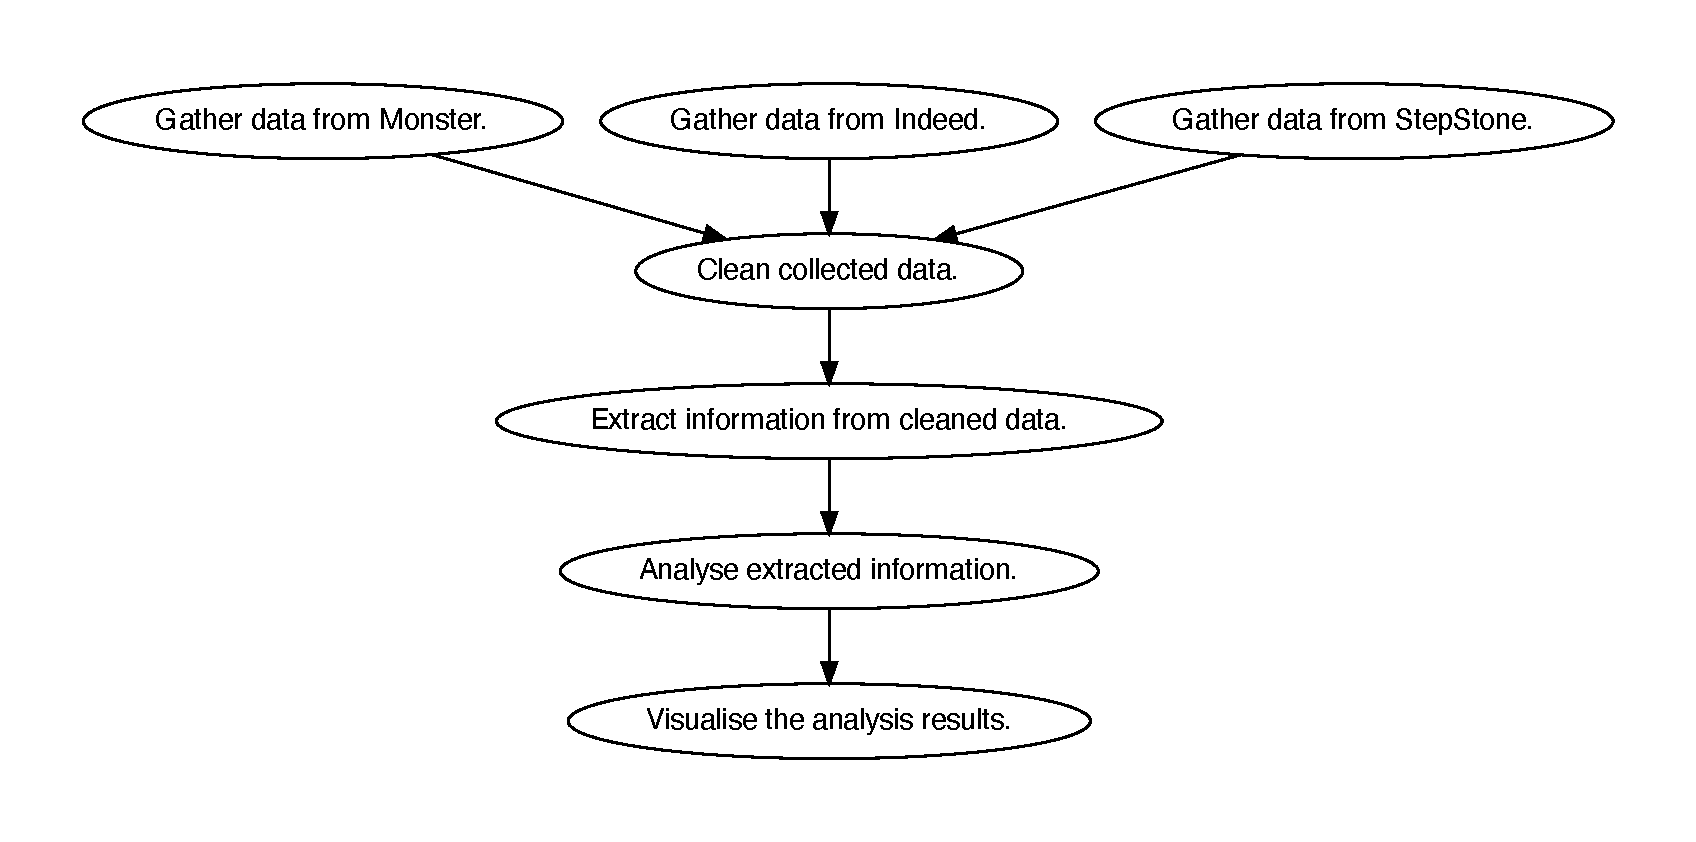
\includegraphics[width=\textwidth]{project-workflow.dot.pdf}
  \end{frame}

  \begin{frame}{Evaluation of Scraping Tools: OctoParse}
    \begin{itemize}
      \item desktop application for scraping
      \item free tier allows scraping unlimited pages on unlimited computers
      \item two concurrent scraping jobs
      \item allows configuring 10 different crawler configurations
      \item only supported on Windows
    \end{itemize}
  \end{frame}

  \begin{frame}{Evaluation of Scraping Tools: ScrapingBot}
    \begin{itemize}
      \item does not provide an application at all
      \item similar to using a proxy server
      \item HTTP request responds with the contents including any rendered JavaScript
      \item free plan only includes 100 API calls per month
    \end{itemize}
  \end{frame}

  \begin{frame}{Evaluation of Scraping Tools: ScrapeStorm}
    \begin{itemize}
      \item desktop application for scraping
      \item works on Linux, macOS as well as Windows
      \item free plan allows 10 different crawler configurations
      \item 1 concurrent local run
      \item allows 100 exported rows per day
    \end{itemize}
  \end{frame}

  \begin{frame}{Evaluation of Scraping Tools: ScrapeStorm Trial}
    \begin{itemize}
      \item scrape Monster detail page
      \item content included in nested \texttt{iframe} element
      \item major problem: extracted content empty
      \item cannot extract nested \texttt{iframe} element
    \end{itemize}
  \end{frame}

  \begin{frame}{Evaluation of Scraping Tools: Selenium \& Firefox}
    \begin{itemize}
      \item supports all of the major web browsers
      \item only thing needed is the so called “webdriver”
      \item can be used with a wide array of programming languages
      \item most importantly: can extract nested \texttt{iframe} elements
    \end{itemize}
  \end{frame}

  \begin{frame}{Implementation}
    \begin{itemize}
      \item Scraping
      \item Natural Language Processing
      \item Data Analysis
    \end{itemize}
  \end{frame}

  \begin{frame}{Implementation: Data Scraping}
    \begin{itemize}
      \item scraping each website consists of two main steps
        \begin{itemize}
          \item perform search request and gather URLs for detail pages
          \item scrape data from detail page
        \end{itemize}
    \end{itemize}
  \end{frame}

  \begin{frame}{Implementation: Data Scraping - Monster URLs}
    \centering
    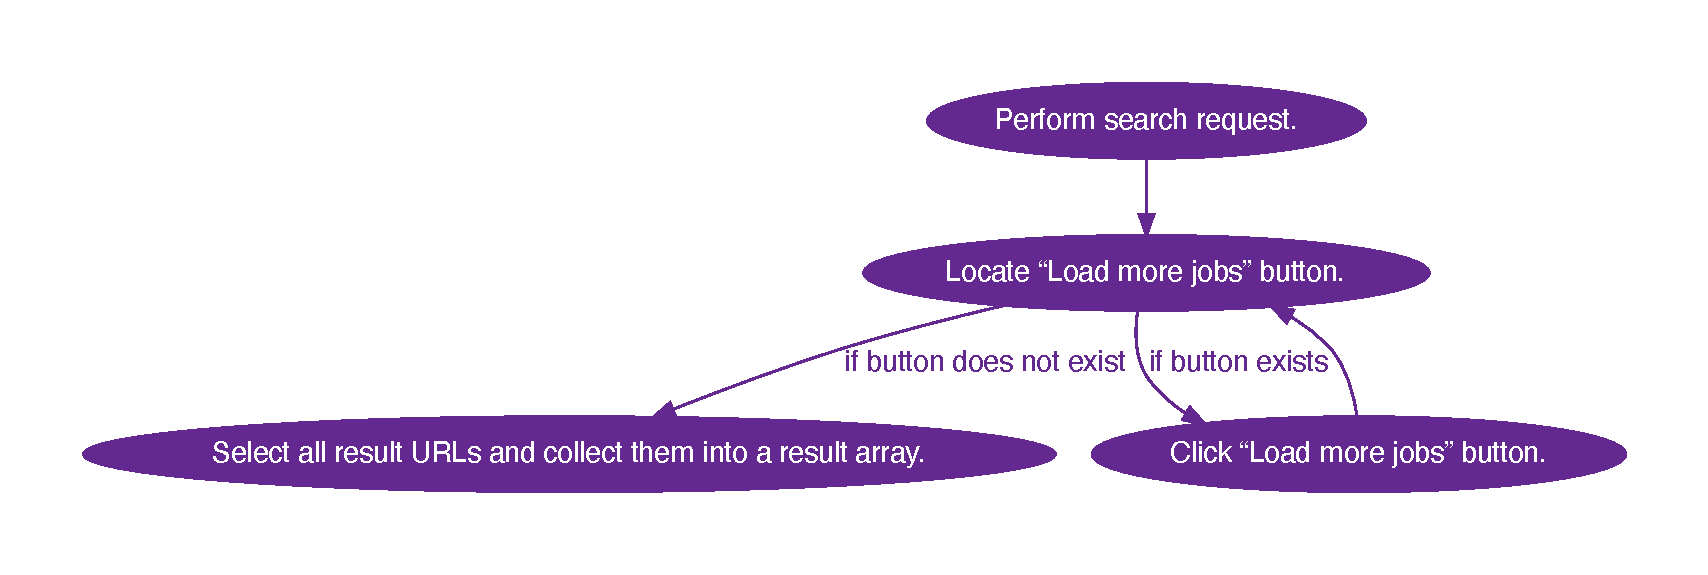
\includegraphics[width=\textwidth]{monster-workflow.dot.pdf}
  \end{frame}

  \begin{frame}{Implementation: Data Scraping - Indeed URLs}
    \centering
    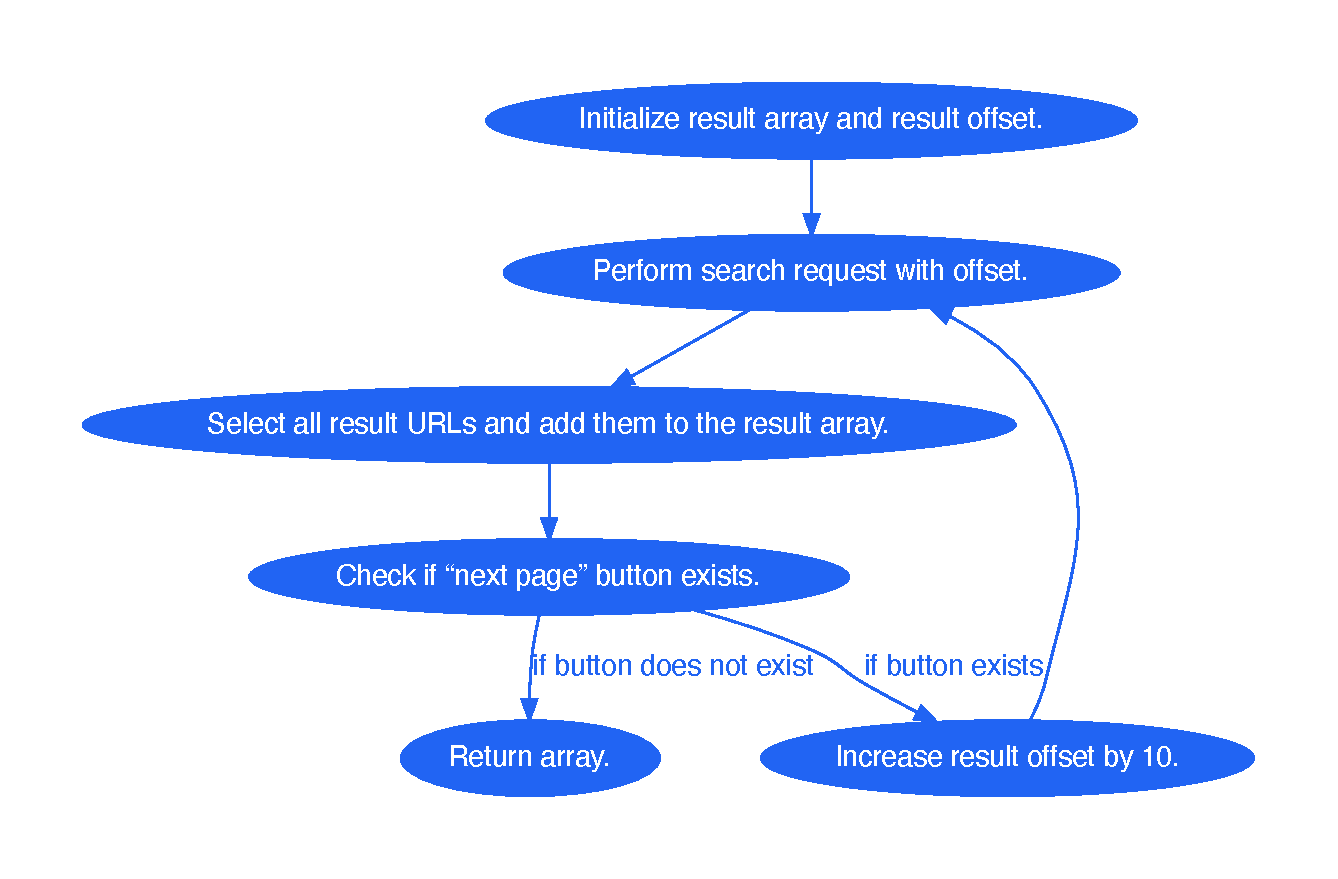
\includegraphics[height=\textheight]{indeed-workflow.dot.pdf}
  \end{frame}

  \begin{frame}{Implementation: Data Scraping - StepStone URLs}
    \centering
    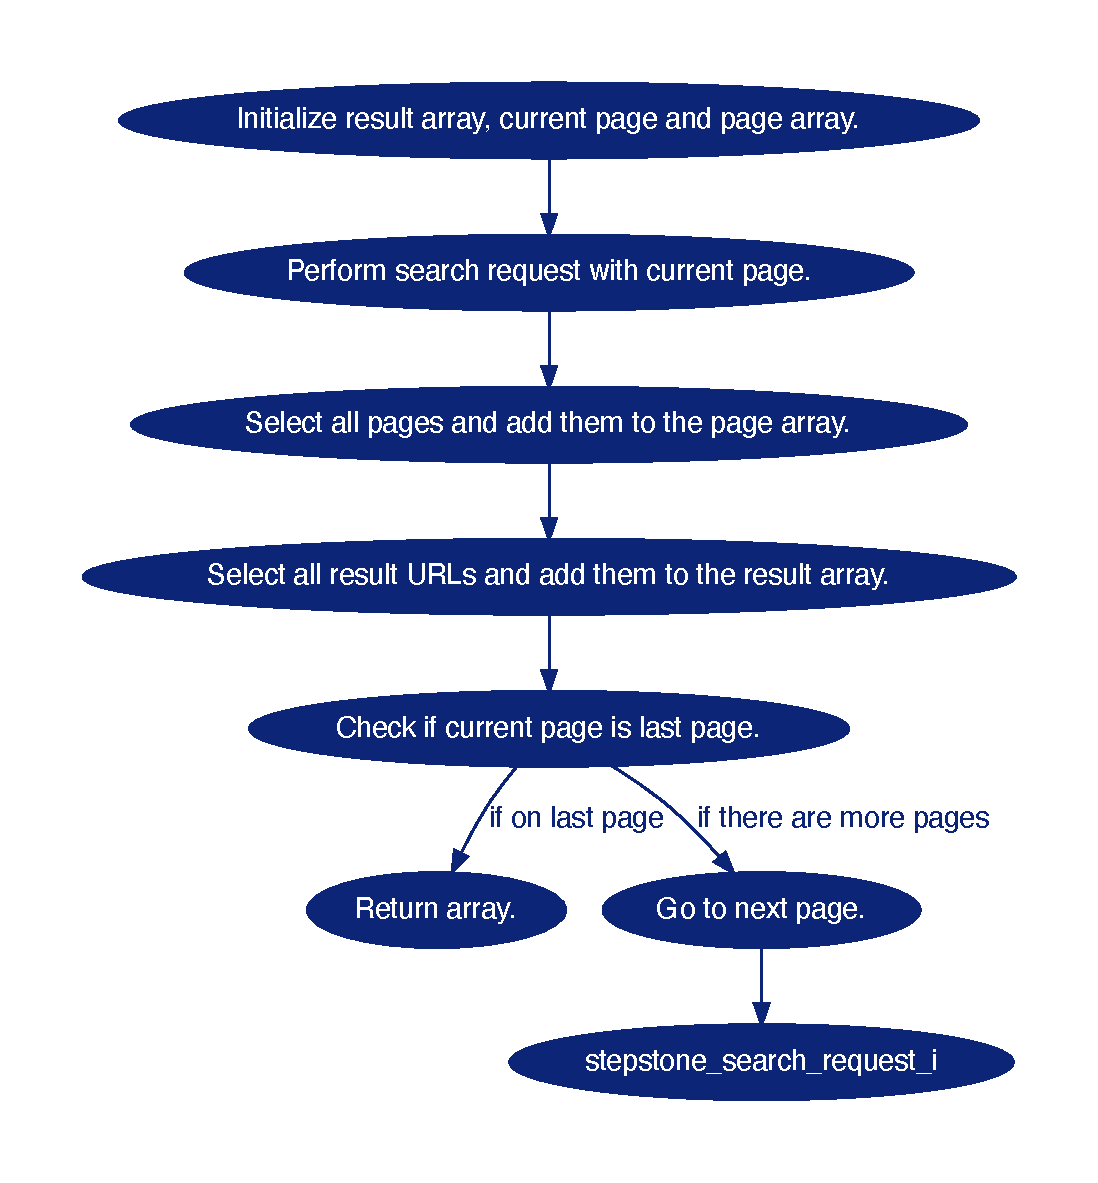
\includegraphics[height=\textheight]{stepstone-workflow.dot.pdf}
  \end{frame}

  \begin{frame}{Implementation: Data Scraping - Detail Page}
    \begin{itemize}
      \item title
      \item metadata: location, contract type
      \item body content on Monster:
        \begin{itemize}
          \item find nested \texttt{iframe} element
          \item use \texttt{switch\_to} function to switch to the \texttt{iframe} element
        \end{itemize}
      \item body content on Indeed and StepStone:
        \begin{itemize}
          \item no nested \texttt{iframe} element
          \item extracted the same way as all other fields
        \end{itemize}
    \end{itemize}
  \end{frame}

  \begin{frame}{Implementation: Natural Language Processing}
    \begin{itemize}
      \item implemented in Python
      \item tokenisation using NLTK (Natural Language Toolkit)
      \item Austrian cities database from \href{https://simplemaps.com}{simplemaps.com}
    \end{itemize}
  \end{frame}

  \begin{frame}{Implementation: Natural Language Processing - Extracted Data}
    \begin{itemize}
      \item average salary
      \item location (including mapping cities to states)
      \item employment type (full-time vs. part-time and permanent vs. temporary)
      \item required education (Matura, bachelor's degree, master's degree etc.)
      \item required certifications
    \end{itemize}
  \end{frame}

  \begin{frame}{Implementation: Natural Language Processing - Example Salary}
    \begin{multicols}{3}
      43,595 Euros \\
      30k Euros \\
      3,100.00 EUR \\
      EUR 2.800,- \\
      EUR 50k \\
      EUR 5700 \\
      EUR 2.600,00 \\
      70.000 € \\
      € 4.209,- \\
      € 3.933,0 \\
      € 55.000,-- \\
      € 65.000,--- \\
      65,000 € \\
      €60,000 \\
      €85k \\
      €3.007,20 \\
      80.000 Euro \\
      60000 €
    \end{multicols}

    \begin{itemize}
      \item needed to be normalised to XXXXX.XX € format
      \item extracted using 2-grams with number and € symbol
    \end{itemize}
  \end{frame}

  \begin{frame}{Implementation: Data Analysis}
    \begin{itemize}
      \item Jupyter Notebook (interactive Python environment)
        \begin{itemize}
          \item very useful for quickly iterating over revisions
          \item graphs are displayed in the same environment as the code
        \end{itemize}
      \item pandas framework for manipulating data
      \item Plotly for generating graphs
    \end{itemize}
  \end{frame}

  \begin{frame}{Findings}
    \begin{itemize}
      \item search term “information security”
      \item 1538 scraped jobs in total
      \begin{itemize}
        \item 993 from Monster
        \item 282 from Indeed
        \item 263 from StepStone
      \end{itemize}
      \item 121 actual information security jobs
        \begin{itemize}
          \item filtered according to job title
        \end{itemize}
    \end{itemize}
  \end{frame}

  \begin{frame}{Findings: Employment Type}
    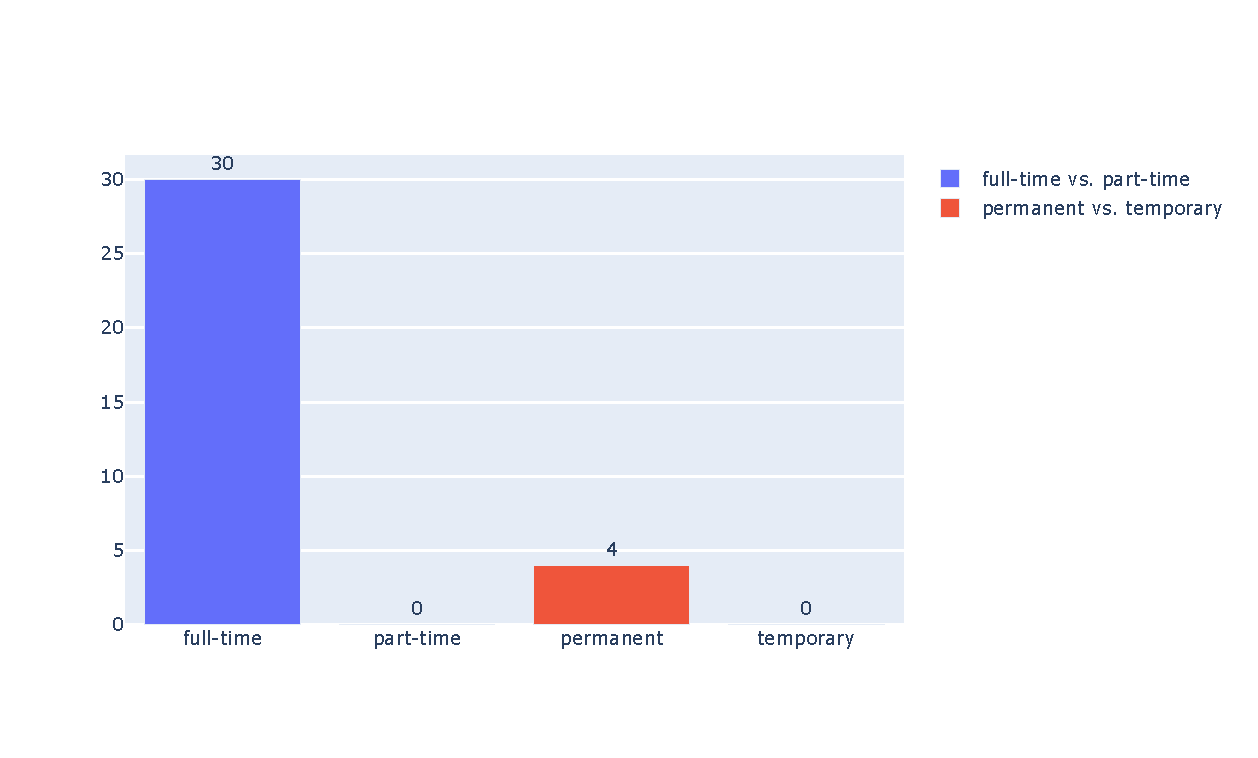
\includegraphics[width=\textwidth]{employment-type-bar-chart.pdf}
  \end{frame}

  \begin{frame}{Findings: Education Type}
    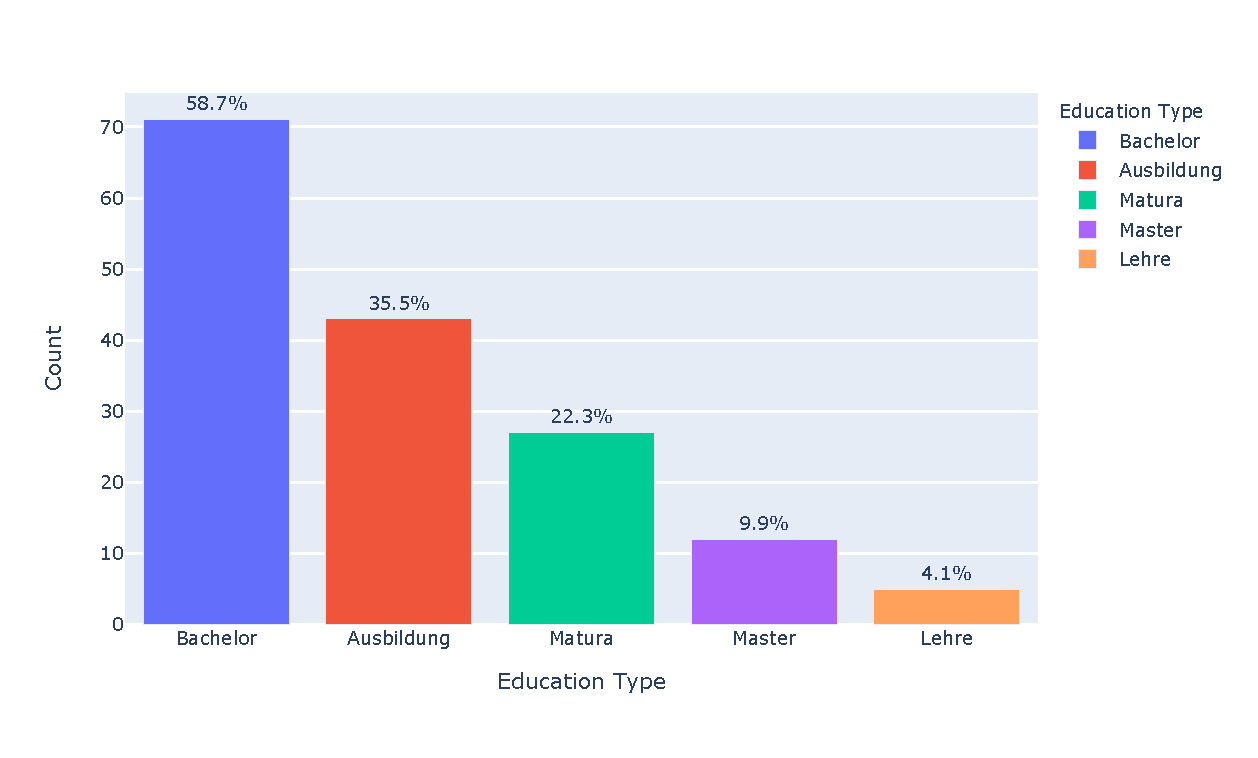
\includegraphics[width=\textwidth]{education-bar-chart.pdf}
  \end{frame}

  \begin{frame}{Findings: Location}
    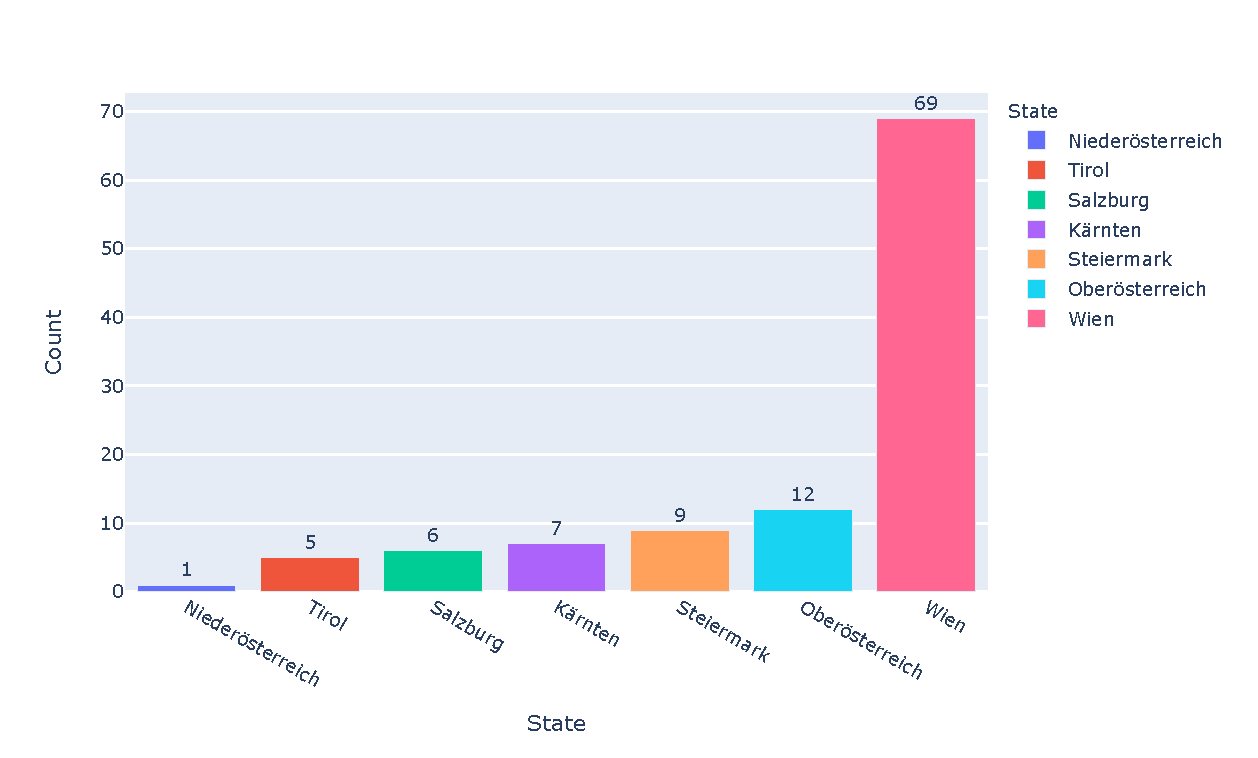
\includegraphics[width=\textwidth]{location-bar-chart.pdf}
  \end{frame}

  \begin{frame}{Findings: Location per Capita}
    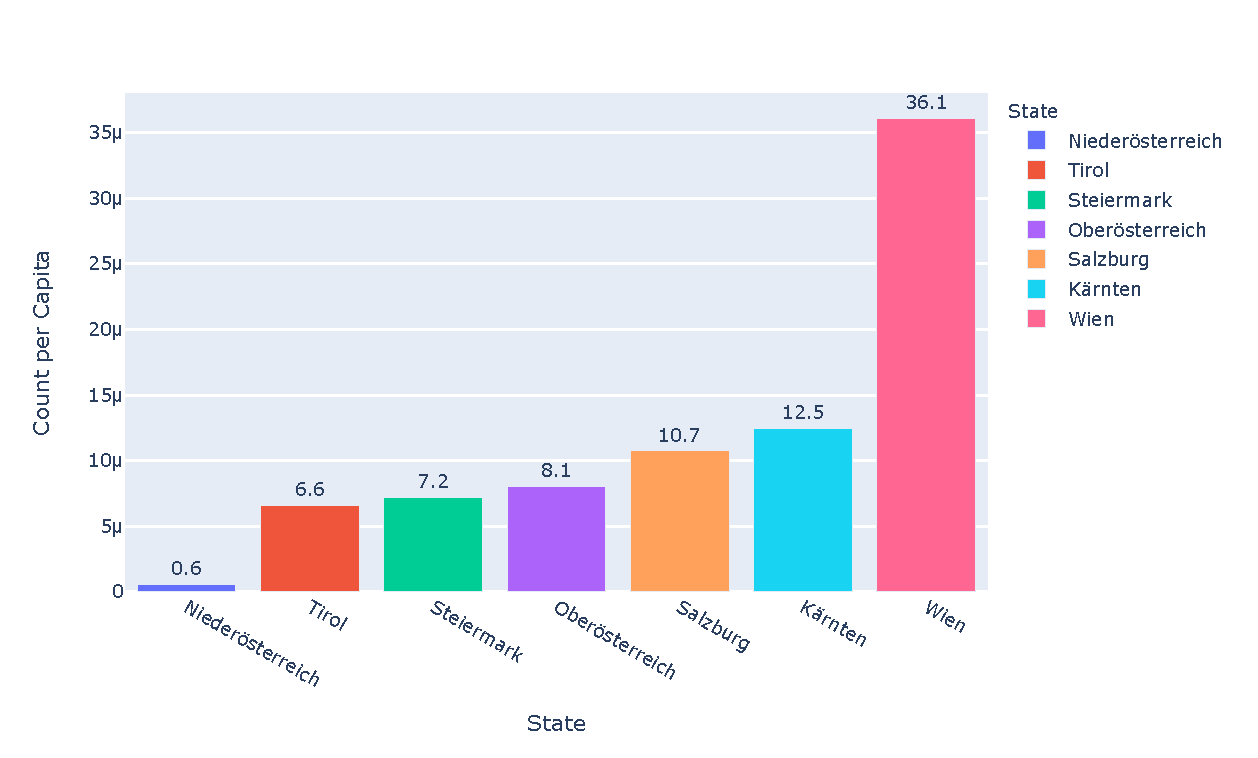
\includegraphics[width=\textwidth]{location-per-capita-bar-chart.pdf}
  \end{frame}

  \begin{frame}{Findings: Average Salary}
    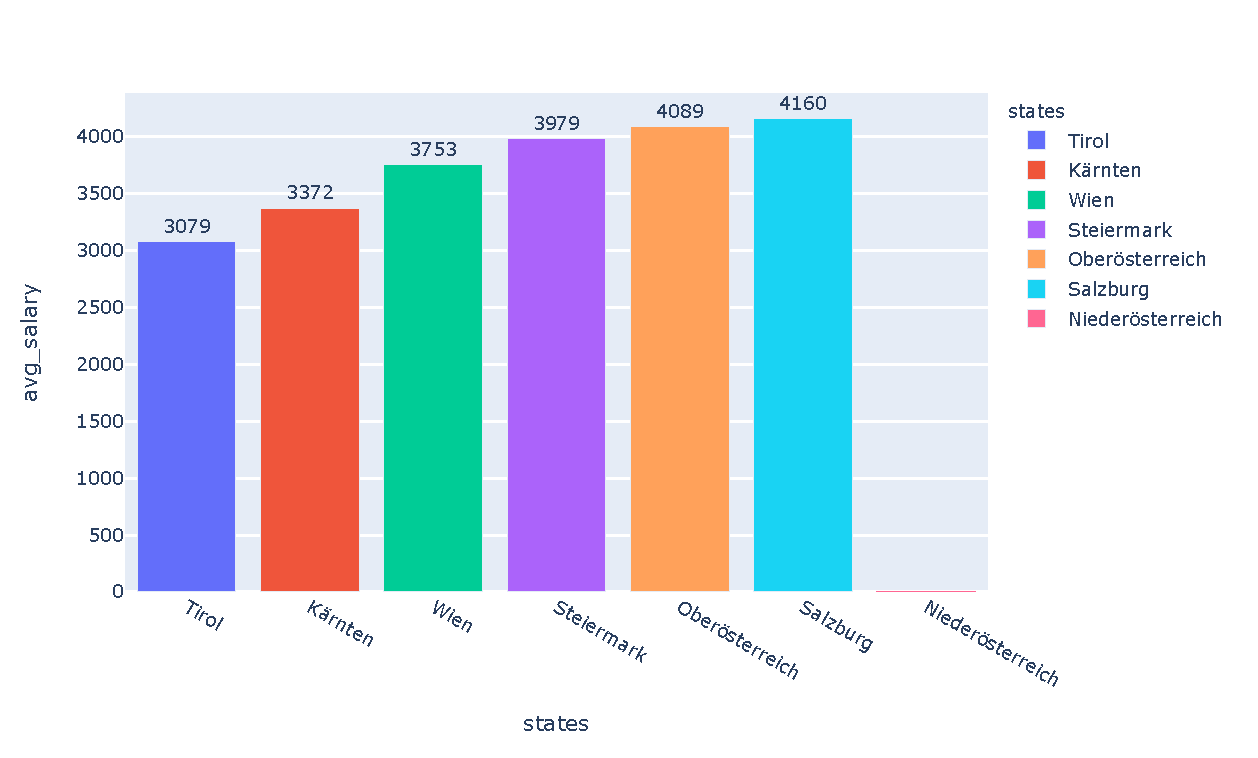
\includegraphics[width=\textwidth]{average-salary-bar-chart.pdf}
  \end{frame}

  \begin{frame}{Findings: Certifications}
    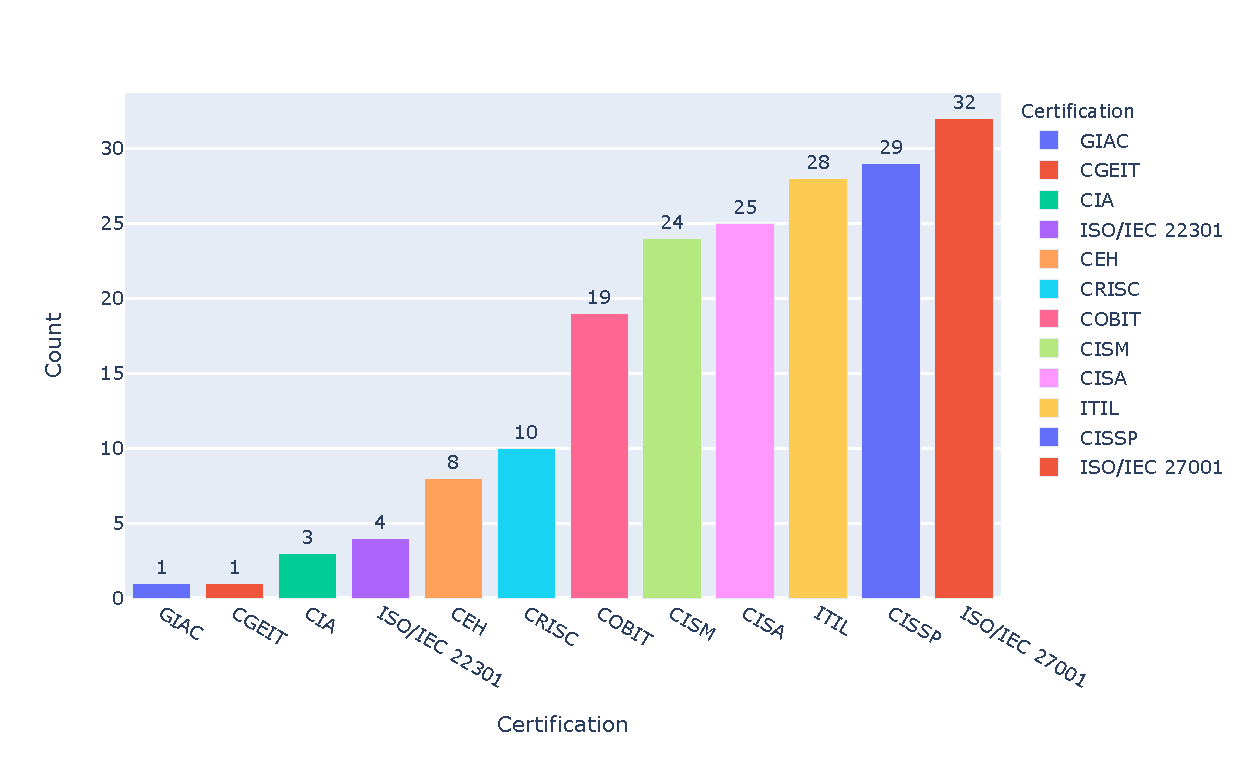
\includegraphics[width=\textwidth]{certifications-bar-chart.pdf}
  \end{frame}

  \begin{frame}{Conclusion}
    \begin{itemize}
      \item compared multiple scraping tools
      \item developed a program for scraping data from three job search sites
      \item findings can be used to inform new decisions on what should be taught in universities
      \item more data points could be implemented in a future revision of this survey
      \item survey could be conducted again within a longer time span
      \item survey could be conducted again with additional job search websites
    \end{itemize}
  \end{frame}
\end{document}
